\documentclass[12pt]{article}

\usepackage{fullpage}
\usepackage{multicol,multirow}
\usepackage{tabularx}
\usepackage{ulem}
\usepackage[utf8]{inputenc}
\usepackage[russian]{babel}
\usepackage{listings}
\usepackage{hyperref}
\usepackage{graphicx}
\DeclareGraphicsExtensions{.png}


\begin{document}

\section*{Лабораторная работа №\,3 по курсу криптографии}

Выполнила студентка группы М8О-307Б \textit{Довженко Анастасия}.

\subsection*{Условие}
\begin{enumerate}
\item Строку в которой записано своё ФИО подать на вход в хеш-функцию ГОСТ Р 34.11-2012 (Стрибог). Младшие 4 бита выхода интерпретировать как число, которое в дальнейшем будет номером варианта. Процесс выбора варианта требуется отразить в отчёте.
\item Программно реализовать один из алгоритмов функции хеширования в соответствии с номером варианта. Алгоритм содержит в себе несколько раундов.
\item Модифицировать оригинальный алгоритм таким образом, чтобы количество раундов было настраиваемым параметром программы. в этом случае новый алгоритм не будет являться стандартом, но будет интересен для исследования.
\item Применить подходы дифференциального криптоанализа к полученным алгоритмам с разным числом раундов.
\item Построить график зависимости количества раундов и возможности различения отдельных бит при количестве раундов 1,2,3,4,5,... .
\item Сделать выводы.
\end{enumerate}

\subsection*{Метод решения}
Выбор варианта с помощью консольной утилиты, взятой из github.com/adegtyarev/streebog:\\
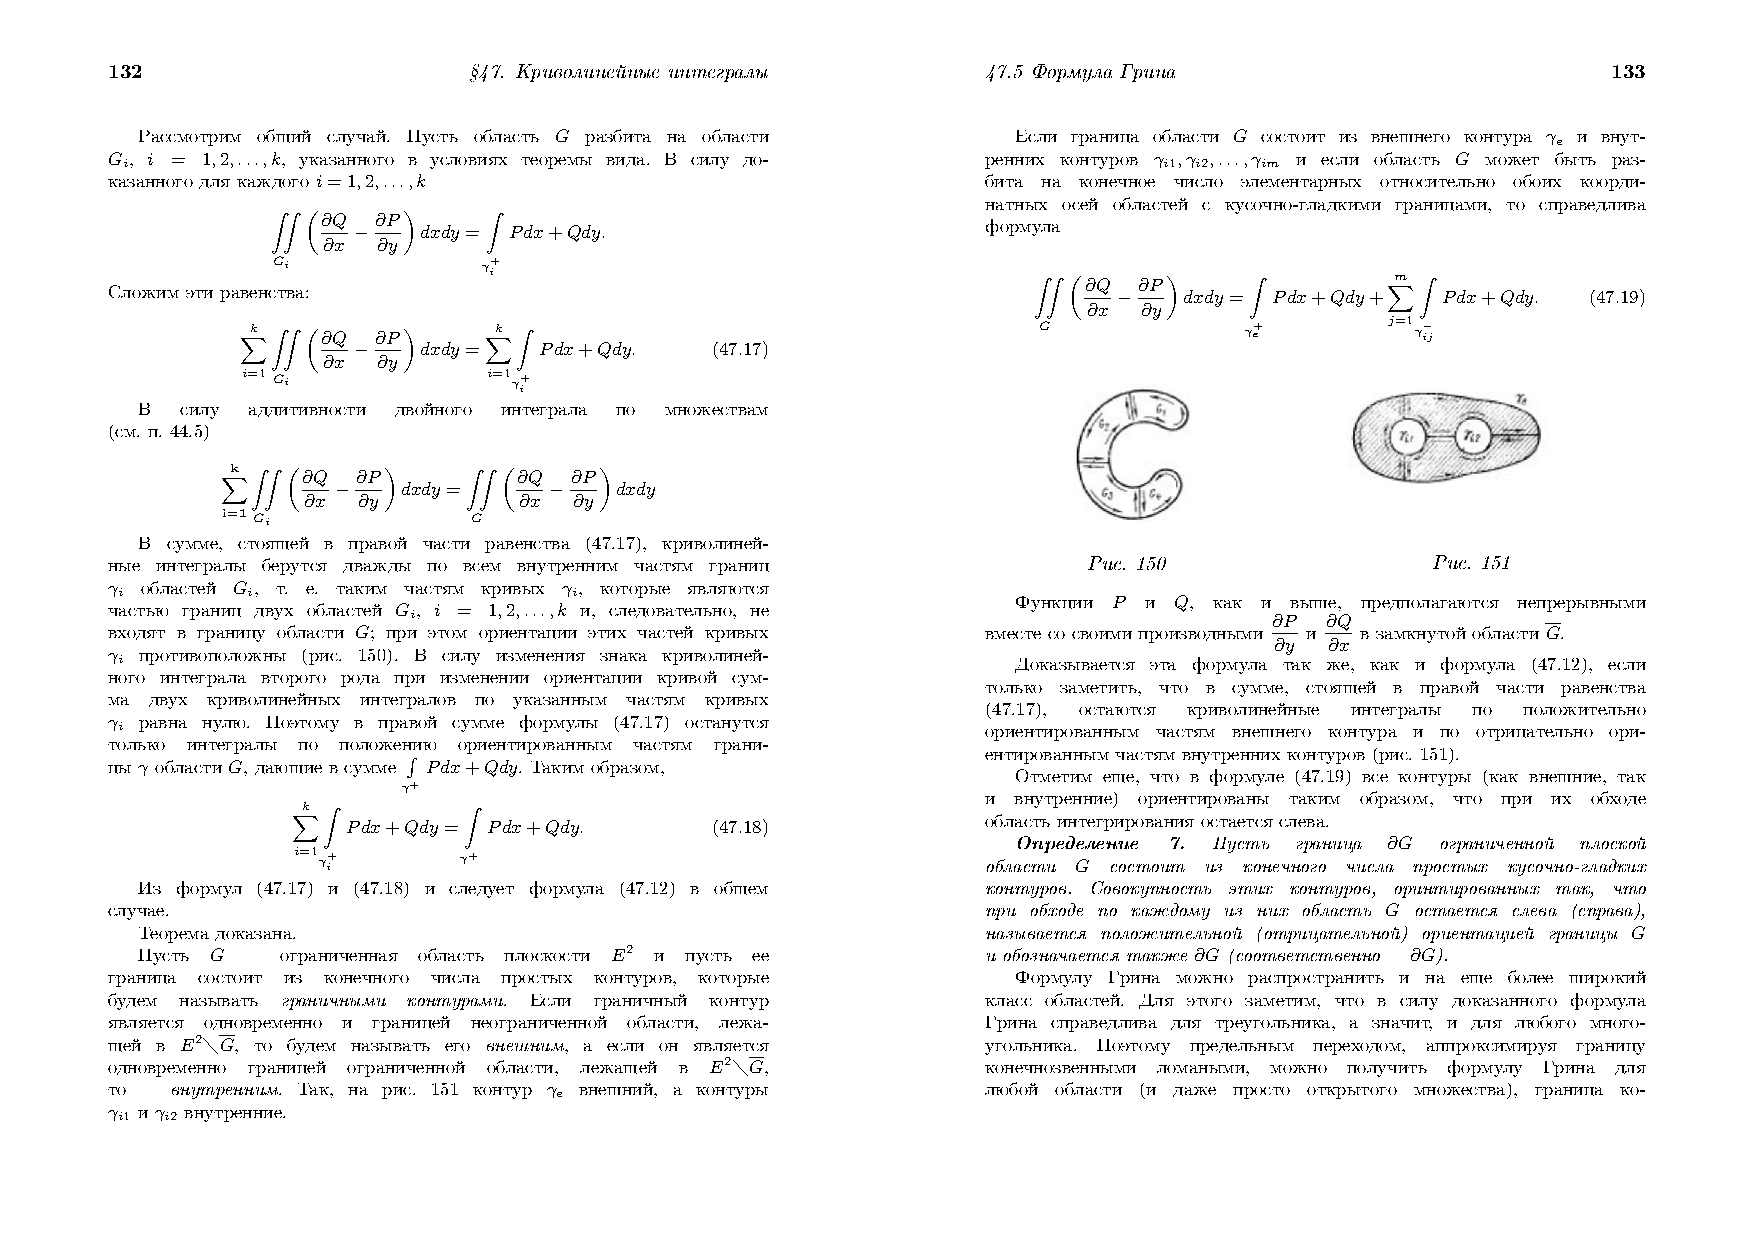
\includegraphics[width=\linewidth]{1.png}\\

\textbf{Вариант 5: SHA-1}

Для выполнения задания было решено написать свою реализацию. SHA-1 работает следующим образом. Сначала происходит препроцессинг исходного сообщения так, чтобы его длина была кратна 512 (это размер блока в алгоритме). К сообщению добвляется 1 бит, затем последовательность 0, чтобы длина последнего блока стала равной 448 бит. В конце дописывается длина исходного сообщения до препроцессинга. Сообщение разбивается на блоки по 512 бит. 
Инициализируются 5 перменных:\\
$h0 = a = 0x67452301$ \\
$h1 = b = 0xEFCDAB89$ \\
$h2 = c = 0x98BADCFE$ \\
$h3 = d = 0x10325476$ \\
$h4 = e = 0xC3D2E1F0$ \\

Определяются четыре функции и четыре константы:\\
$ F_{t}(m, l, k) = (m \& l) \mid (\sim m \& k), K_{t} = 0x5A827999, 0 \leq t \leq 19$\\
$ F_{t}(m, l, k) = m \oplus l \oplus k, K_{t} = 0x6ED9EBA1, 20 \leq t \leq 39$\\
$ F_{t}(m, l, k) = (m \& l) \mid (m \& k) \mid  (l \& k), K_{t} = 0x8F1BBCDC, 40 \leq t \leq 59$\\
$ F_{t}(m, l, k) = m \oplus l \oplus k, K_{t} = 0xCA62C1D6, 60 \leq t \leq 79$\\

В главном цикле итеративно обрабатываются все 512-битные блоки. Согласно стандарту, проводится 80 раундов. Блок сообщения преобразуется из 16 32-битовых слов $M_{i}$ в 80 32-битовых слов $W_{j}$ по следующему правилу: \\
$W_{t} = M_{t}, 0 \leq t \leq 15 $\\
$W_{t} = (W_{t-3} \oplus W_{t-8} \oplus W_{t-14} \oplus W_{t-16}) \ll 1, 16 \leq t \leq 79$\\

Далее вычисляются функции, описанные выше. В конце каждого раунда обновляются $a, b, c, d, e$:\\
$ temp = (a \ll 5) + F_{t}(b, c, d) + W_{t} + K_{t} $\\
$ e = d $ \\
$ d = c $ \\
$ c = b \ll 30 $ \\
$ b = a $ \\
$ a = temp $ \\

После обработки блока $a, b, c, d, e$ прибавляются к $h0, h1, h2, h3, h4$ соответственно. Начинается следующая итерация. Итоговым значением будет объединение пяти 32-битовых слов в одно 160-битное хеш-значение.

\par
Реализация проходит все юнит тесты. Я сделала два вида тестов. Первый проверяет, что для одного и того же входного сообщения мой SHA-1 получает одинаковые хеш-значения. Второй сравнивает хеш-значение, полученное моей функцией, со значением, полученным функцией из стандартной библиотеки. \par

\par
Далее были применены подходы дифференциального криптоанализа к полученной хеш-функции. Я генерирую строку, создаю ее копию с инвертированным последним битом. Затем считаю хеши обеих строк для количества раундов в интервале от 0 до 80 с шагом 5. В конце считаю количество различных бит в полученных хешах. Для более честного анализа данная процедура была проведена 10 раз и взяты средние значения количества измененных бит для каждого теста с раундами. \par


\begin{tabular}{ | c | c | }
\hline
Кол-во раундов & Число изменных бит \\ \hline
5 & 0 \\ \hline
10 & 0 \\ \hline
15 & 8 \\ \hline
20 & 55 \\ \hline
25 & 83 \\ \hline
30 & 79 \\ \hline
35 & 80 \\ \hline
40 & 79 \\ \hline
45 & 81 \\ \hline
50 & 79 \\ \hline
55 & 78 \\ \hline
60 & 80 \\ \hline
65 & 81 \\ \hline
70 & 76 \\ \hline
75 & 84 \\ \hline
80 & 80 \\ \hline
\end{tabular}
\\
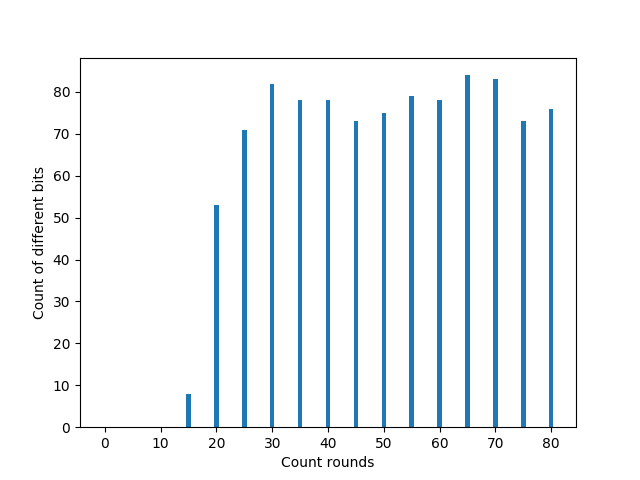
\includegraphics[width=\linewidth]{res.png}\\

Такой анализ позволяет увидеть, насколько меняется хеш при минимальном изменении исходного сообщения. Учитывая, что итоговое значение имеет длину 160 бит, нетрудно заметить, что примерно с 25 раунда меняется примерно половина бит хеша, что не может нас не радовать с точки зрения криптографии. Можно предположить, что SHA-1 удовлетворяет лавинному критерию. Конечно, сложно утверждать, что полученные результаты хоть сколько-нибудь значимы, потому что было проведено слишком мало тестов.

\subsection*{Результат работы программы}
\begin{lstlisting}
karma@mydruzhok:~/mai_study/Crypto/lab3$ python test.py 

>>> test_comparison
... test_comparison: checking for identical digests (random string)
... test_comparison: success
... test_comparison: checking for identical digests (test cases)
... test:  abc
... test:  
... test:  abcdbcdecdefdefgefghfghighijhijkijkljklmklmnlmnomnopnopq
... test:  abcdefghbcdefghicdefghijdefghijkefghijklfghijklmghijklmn
hijklmnoijklmnopjklmnopqklmnopqrlmnopqrsmnopqrstnopqrstu
... test:  a (1,000,000 repetitions)
... test_comparison: success
.
>>> test_repeatable
... test_repeatable: checking for identical digests
... test_repeatable: success
.
----------------------------------------------------------------------
Ran 2 tests in 3.341s

OK
karma@mydruzhok:~/mai_study/Crypto/lab3$ python diff_anal.py 
Count rounds: 0
Count of different bits: 0
------------
Count rounds: 5
Count of different bits: 0
------------
Count rounds: 10
Count of different bits: 0
------------
Count rounds: 15
Count of different bits: 8
------------
Count rounds: 20
Count of different bits: 55
------------
Count rounds: 25
Count of different bits: 83
------------
Count rounds: 30
Count of different bits: 79
------------
Count rounds: 35
Count of different bits: 80
------------
Count rounds: 40
Count of different bits: 79
------------
Count rounds: 45
Count of different bits: 81
------------
Count rounds: 50
Count of different bits: 79
------------
Count rounds: 55
Count of different bits: 78
------------
Count rounds: 60
Count of different bits: 80
------------
Count rounds: 65
Count of different bits: 81
------------
Count rounds: 70
Count of different bits: 76
------------
Count rounds: 75
Count of different bits: 84
------------
Count rounds: 80
Count of different bits: 80
------------
\end{lstlisting}

\subsection*{Выводы}
Мне уже приходилось сталкиваться с хеш-функциями в курсе операционных систем. Тогда я реализовывала Adler-32 и MurmurHash2. В этой лабораторной я познакомилась с криптографическими хеш-функциями, а конкретно с SHA-1. Теперь я могу безопасно и (почти) без коллизий вычислять хеши. SHA1 -- классика, однако существует множество других более надежных, быстрых и устойчивых к атакам хеш-функций. Метод дифференциального криптоанализа показался мне сложен для понимания, думаю это связано с моим поверхностным знакомством с криптоанализом в целом. Но было интересно провести мини-исследование, используя отдельный подход.

\subsection*{Листинг программного кода}
sha1.py
\begin{lstlisting}[language=Python]
import os
import argparse


CNT_ROUNDS = 80
BLOCK_SIZE = 512


class SHA1:
    def __init__(self, rounds):
        self.h = (0x67452301,
                  0xEFCDAB89,
                  0x98BADCFE,
                  0x10325476,
                  0xC3D2E1F0)
        self.rounds = rounds

    def update(self, msg):
        msg_bin = ''
        for i in range(len(msg)):
            msg_bin += '{0:08b}'.format(ord(msg[i]))

        len_msg = len(msg_bin)

        msg_bin += '1'
        while (len(msg_bin) % 512 != 448):
            msg_bin += '0'

        msg_bin += '{0:064b}'.format(len_msg)

        chunks = self.get_chunks(msg_bin)
        for chunk in chunks:
            self.process_chunk(chunk)

        return self

    def hexdigest(self):
        return '%08x%08x%08x%08x%08x' % self.h

    def get_chunks(self, msg):
        return [msg[i:i + BLOCK_SIZE] for i in range(0, len(msg),  \
            BLOCK_SIZE)]

    def process_chunk(self, chunk):
        h0, h1, h2, h3, h4 = (i for i in self.h)

        w = []
        for i in range(16):
            w.append(int(chunk[i * 32:i * 32 + 32], 2))
        for i in range(16, 80):
            w.append(self.rotl(w[i - 3] ^ w[i - 8] ^ w[i - 14] ^ \ 
            w[i - 16], 1))

        a, b, c, d, e = h0, h1, h2, h3, h4

        for i in range(self.rounds):
            if 0 <= i <= 19:
                f = (b & c) | ((~b) & d)
                k = 0x5A827999
            elif 20 <= i <= 39:
                f = b ^ c ^ d
                k = 0x6ED9EBA1
            elif 40 <= i <= 59:
                f = (b & c) | (b & d) | (c & d)
                k = 0x8F1BBCDC
            elif 60 <= i <= 79:
                f = b ^ c ^ d
                k = 0xCA62C1D6

            a, b, c, d, e = (self.rotl(a, 5) + f + e + k + w[i]) & \ 
            0xffffffff, a, self.rotl(b, 30), c, d

        h0 = (h0 + a) & 0xffffffff
        h1 = (h1 + b) & 0xffffffff
        h2 = (h2 + c) & 0xffffffff
        h3 = (h3 + d) & 0xffffffff
        h4 = (h4 + e) & 0xffffffff

        self.h = (h0, h1, h2, h3, h4)

    @staticmethod
    def rotl(n, k):
        return ((n << k) | (n >> (32 - k))) & 0xffffffff


def sha1(msg, rounds):
    return SHA1(rounds).update(msg).hexdigest()


if __name__ == '__main__':
    parser = argparse.ArgumentParser()
    parser.add_argument('--rounds', help='Count rounds (<= 80)')
    parser.add_argument('--input', required=True, 
                        help='Input file to hash')
    args = parser.parse_args()

    rounds = int(args.rounds) if args.rounds else CNT_ROUNDS
    filename = args.input
    if os.path.isfile(filename):
        with open(filename, "r") as f:
            text = f.read()
            print('sha1: ', sha1(text, rounds))
    else:
        print("Error, could not find " + filename + " file." )

\end{lstlisting}

test.py
\begin{lstlisting}[language=Python]
import unittest
import random
import string
import hashlib

import sha1


CNT_ROUNDS = 80


class TestSha1(unittest.TestCase):
    def test_repeatable(self):
        print('\n>>> test_repeatable')
        msg = get_random_string()

        first_digest = sha1.sha1(msg, CNT_ROUNDS)
        second_digest = sha1.sha1(msg, CNT_ROUNDS)

        print('... test_repeatable: checking for identical digests')
        self.assertEqual(first_digest, second_digest)
        print('... test_repeatable: success')

    def test_comparison(self):
        print('\n>>> test_comparison')
        msg = get_random_string()

        custom_sha1 = sha1.sha1(msg, CNT_ROUNDS)
        lib_sha1 = hashlib.sha1(msg.encode()).hexdigest()

        print('... test_comparison: checking for identical 
                digests (random string)')
        self.assertEqual(custom_sha1, lib_sha1)
        print('... test_comparison: success')

        tests = ('abc', '', 'abcdbcdecdefdefgefghfghighijh
            ijkijkljklmklmnlmnomnopnopq', \
            'abcdefghbcdefghicdefghijdefg \ 
            hijkefghijklfghijklmghijklmnh \
            ijklmnoijklmnopjklmnopqklmnop \
            qrlmnopqrsmnopqrstnopqrstu', \
            'a' * 1000000)

        print('... test_comparison: checking for identical 
                digests (test cases)')
        for test in tests:
            print('... test: ', test if len(test) < 10**6 else \ 
                    'a (1,000,000 repetitions)')
            custom_sha1 = sha1.sha1(test, CNT_ROUNDS)
            lib_sha1 = hashlib.sha1(test.encode()).hexdigest()
            self.assertEqual(custom_sha1, lib_sha1)
        print('... test_comparison: success')


def get_random_string():
    return ''.join(random.choice(string.ascii_letters + string.digits) 
                    for _ in range(random.randint(10, 10 ** 5)))


if __name__ == '__main__':
    unittest.main()
\end{lstlisting}

diff\_anal.py
\begin{lstlisting}[language=Python]
import random
import string
import logging

import bitarray
import matplotlib.pyplot as plt

import sha1


CNT_TESTS = 11


def get_random_string(N=50):
    return ''.join(random.choice(string.ascii_letters + string.digits)
            for _ in range(N))


def change_one_bit(msg):
    ba = bitarray.bitarray()
    ba.frombytes(msg.encode('ascii'))
    last_bit = ba[-1]
    new_last = bitarray.bitarray('0') if last_bit else \ 
                bitarray.bitarray('1')
    ba = ba[:-1]
    ba += new_last
    return bitarray.bitarray(ba.tolist()).tobytes().decode('ascii')


def bitcount(n):
    return bin(n).count('1')


def mean(list_):
    return [int(sum(i) / len(i)) for i in zip(*list_)]


if __name__ == '__main__':
    logging.basicConfig(filename="analysis.log", level=logging.INFO)

    all_diffs = []
    cnt_rounds = [i for i in range(0, 81, 5)]
    for i in range(1, CNT_TESTS):
        logging.info("Test #{0}".format(i))
        input1 = get_random_string()
        input2 = change_one_bit(input1)

        logging.info("Input string:   {0}".format(input1))
        logging.info("Changed string: {0}".format(input2))

        diffs = []
        rounds = range(0, 81, 5)
        for i in rounds:
            logging.info("Count rounds: ".format(i))
            output1 = sha1.sha1(input1, i)
            output2 = sha1.sha1(input2, i)
            logging.info("Output original:  {0}".format(output1))
            logging.info("Output changed:   {0}".format(output2))
            res = bitcount(int(output1, 16) ^ int(output2, 16))
            diffs.append(res)
            logging.info("Count of different bits: {0}".format(res))
        logging.info("------------")
        all_diffs.append(diffs)

    mean_diffs = mean(all_diffs)
    for i, j in zip(cnt_rounds, mean_diffs):
        print("Count rounds: {0}".format(i))
        print("Count of different bits: {0}".format(j))
        print("------------")

    plt.bar(cnt_rounds, mean_diffs, align='center')
    plt.xlabel('Count rounds')
    plt.ylabel('Count of different bits')
    plt.show()
\end{lstlisting}

\end{document}
